\documentclass[a4,paper,fleqn]{article}

\usepackage{../../layout/layout}

\title{Notizen DSVB -- SW02}
\date{\today}
\author{Daniel Winz}

\begin{document}
\maketitle
\clearpage

\section{Quantisierungsmodell}
\[ SNR_{\si{\deci\bel}} = 10 \cdot \log_{10} = \left(\frac{P_X}{P_\epsilon}\right) = 6 \cdot W + \delta \approx 6 \cdot W \]
\begin{itemize}
    \item Nutzsignal harmonisches Sinussignal
    \item Nutzsignal vollständig ausgesteuert
\end{itemize}
$\to$ Mit jedem zusätzlichen Bit wird der Signal-Rausch-Abstand um 6\si{\deci\bel} erhöht. 

\section{Matlab Befehle}
\begin{table}[h!]
    \begin{zebratabular}{ll}
        \rowcolor{gray} Befehl & Funktion \\
        \verb!load(spf1);! & Variable spf1 laden \\
        \verb!sound(spf1);! & Daten abspielen \\
        \verb!sound(spf1,Fs);! & Daten abspielen mit Abtastrate \verb!Fs! \\
    \end{zebratabular}
\end{table}

\section{Quantisierung in Matlab}
\begin{tabular}{ccc}
$x[n]$   & \verb!X.XXXXXX!                 & $[-1,+1)$ \\\\
         & $\Downarrow \cdot 2^{(W - 1)}$  & \\\\
         & \verb!XXXX.XXX!                 & $[-1,+1)$ \\\\
         & $\Downarrow$ \verb!round()!     & \\\\
         & \verb!XXXX.   !                 & $[-1,+1)$ \\\\
         & $\Downarrow \cdot 2^{-(W - 1)}$ & \\\\
$X_q[n]$ & \verb!X.XXX   !                 & $[-1,+1)$ \\\\
\end{tabular}

\clearpage

\section{Runden in Matlab}
\begin{figure}[h!]
    \begin{minipage}[c]{0.5\textwidth}
        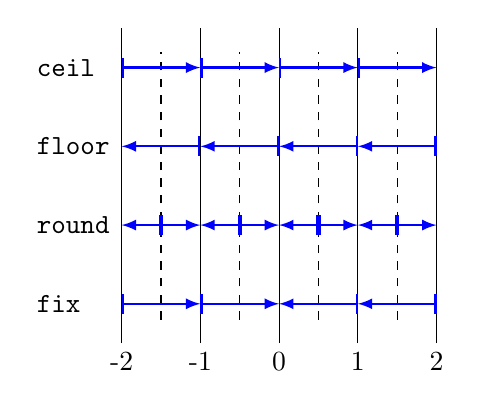
\begin{tikzpicture}
            \draw[] (1,-0.5) node[below] {-2} -- (1,3.5);
            \draw[] (2,-0.5) node[below] {-1} -- (2,3.5);
            \draw[] (3,-0.5) node[below] { 0} -- (3,3.5);
            \draw[] (4,-0.5) node[below] { 1} -- (4,3.5);
            \draw[] (5,-0.5) node[below] { 2} -- (5,3.5);
            \draw[dashed] (1.5,-0.2) -- (1.5,3.2);
            \draw[dashed] (2.5,-0.2) -- (2.5,3.2);
            \draw[dashed] (3.5,-0.2) -- (3.5,3.2);
            \draw[dashed] (4.5,-0.2) -- (4.5,3.2);
            \node at (-0.2,3) [right] {\verb!ceil!};
            \draw[|-latex, blue, thick] (1,3) -- (2,3);
            \draw[|-latex, blue, thick] (2,3) -- (3,3);
            \draw[|-latex, blue, thick] (3,3) -- (4,3);
            \draw[|-latex, blue, thick] (4,3) -- (5,3);
            \node at (-0.2,2) [right] {\verb!floor!};
            \draw[|-latex, blue, thick] (2,2) -- (1,2);
            \draw[|-latex, blue, thick] (3,2) -- (2,2);
            \draw[|-latex, blue, thick] (4,2) -- (3,2);
            \draw[|-latex, blue, thick] (5,2) -- (4,2);
            \node at (-0.2,1) [right] {\verb!round!};
            \draw[|-latex, blue, thick] (1.5,1) -- (1,1);
            \draw[|-latex, blue, thick] (1.5,1) -- (2,1);
            \draw[|-latex, blue, thick] (2.5,1) -- (2,1);
            \draw[|-latex, blue, thick] (2.5,1) -- (3,1);
            \draw[|-latex, blue, thick] (3.5,1) -- (3,1);
            \draw[|-latex, blue, thick] (3.5,1) -- (4,1);
            \draw[|-latex, blue, thick] (4.5,1) -- (4,1);
            \draw[|-latex, blue, thick] (4.5,1) -- (5,1);
            \node at (-0.2,0) [right] {\verb!fix!};
            \draw[|-latex, blue, thick] (1,0) -- (2,0);
            \draw[|-latex, blue, thick] (2,0) -- (3,0);
            \draw[|-latex, blue, thick] (4,0) -- (3,0);
            \draw[|-latex, blue, thick] (5,0) -- (4,0);
        \end{tikzpicture}
    \end{minipage}
    \begin{minipage}[c]{0.5\textwidth}
        \includegraphics[width = 1.0\textwidth]{round_matlab.pdf}
    \end{minipage}
\end{figure}

\section{DFT}
\[ \cos(2 \pi \cdot \underbrace{f}_{k \cdot \frac{f_s}{N}} \cdot \underbrace{t}_{n \cdot T_s}) \]
\[ \cos\left(2 \pi \cdot \frac{k}{N} \cdot n\right) \]

\section{DFT als Korrelation}
\[ X[k] = 
        \sum\limits_{n = 0}^{N} x[n] \cdot     \cos\left(2 \pi \cdot n \cdot \frac{k}{N}\right) + 
j \cdot \sum\limits_{n = 0}^{N} x[n] \cdot (-1)\sin\left(2 \pi \cdot n \cdot \frac{k}{N}\right) + 
\]
\end{document}
